%\documentclass[11pt]{article}
\documentclass[answers]{exam}

\usepackage{amsmath}
%\usepackage{extsizes}
\usepackage{amsmath,amssymb}
%\usepackage{omegavn,ocmrvn}
%\usepackage[utf8x]{inputenc}
\usepackage[utf8]{vietnam}
\DeclareUnicodeCharacter{00A0}{ }

\usepackage{longtable}
\usepackage{answers}
\usepackage{graphicx}
\usepackage{array}
\usepackage{pifont}
\usepackage{picinpar}
\usepackage{enumerate}
\usepackage[top=3.0cm, bottom=3.5cm, left=3.5cm, right=2.5cm] {geometry}
\usepackage{hyperref}


\newtheorem{bt}{Câu}
\newcommand{\RR}{\mathbb R}
\Newassociation{sol}{Solution}{ans}
\newtheorem{ex}{Câu}
\renewcommand{\solutionstyle}[1]{\textbf{ #1}.}


\begin{document}
% \noindent
\begin{tabular*}
{\linewidth}{c>{\centering\hspace{0pt}} p{.7\textwidth}}
Trường ĐHKHTN, ĐHQGHN & {\bf Học Kỳ 1 (2019-2020)}
\tabularnewline
K62 TTƯD & {\bf Bài Tập Giải Tích Số. No 1}
\tabularnewline
\rule{1in}{1pt}  \small  & \rule{2in}{1pt} %(Due date:)
\tabularnewline

%  \tabularnewline
%  &(Đề thi có 1 trang)
\end{tabular*}
%
%\Opensolutionfile{ans}[ans1]
\printanswers

\centering{BÀI TẬP THỰC HÀNH TRÊN LỚP}

\begin{bt}\label{bt1}
Xem bài tập 1 (sách giáo trình - PKA) trang 31. \\
i) Hãy tính số e tới chính xác tới 8 chữ số sau dấu chấm thập phân. Sử dụng thuật toán trang 31, hãy viết script trong Python. \\
ii) Câu hỏi tương tự đối với hàm $\ln(x+1)$.
\end{bt}

\begin{bt}
	Ba số hạng khác không đầu tiên trong khai triển Maclaurin của hàm $arctan$ là $x - (1/3)x^3 + (1/5)x^5$. Hãy tính sai số tuyệt đối và sai số tương đối của $\pi$ bằng cách sử dụng đa thức đó để xấp xỉ hàm $arctan$ đến 6 chữ số thập phân trong các biểu thức sau. Viết script để tính toán trong Python.
	%
	\begin{equation*} 
	a.\ 4 \ (\arctan \frac{1}{2} + arctan \frac{1}{3}) \hskip 2cm b.\ 16 \ arctan \frac{1}{5} - 4 \ arctan \frac{1}{239}.
	\end{equation*}
	%
\end{bt}

\begin{bt}
	Cho hàm số $f(x) = \dfrac{x cos x - sin x}{x - sin x}$. Viết script để tính toán trong Python các phần b, c, d.\\
	a. Tìm $\underset{x \rightarrow 0}{\lim} f(x)$. \\
	b. Tính $f(0.1)$ chính xác đến 6 chữ số thập phân, dùng các hàm sin, cos có sẵn. \\
	c. Hãy thay thế các hàm lượng giác trong công thức của $f(x)$ bằng khai triển Maclaurin bậc 3 (chứa $x^3$) và thực hiện lại phần (b). \\
	d. Cho giá trị chính xác của $f (0.1)=-1.99899998$. Xác định sai số tương đối của các xấp xỉ trong 2 phần (b) và (c).	
\end{bt}

\begin{bt} a) Ôn lại thuật toán Horner. Viết script Python để tính các đa thức sau một cách hiệu quả.
$p_1(x) = 3(x-1)^5+7(x-1)^9$, \quad $p_2(x) = 6(x+2)^3 + 9(x+2)^7 + 3 (x+2)^{15} - (x+2)^{31}.$	 \\
	
b) Viết script tìm thương và số dư của phép chia đa thức $p(x)=a_nx^n+...+a_0$ cho đa thức $x-r$.
Test script cho $p(x)=x^4-4x^3+7x^2-5x-3$ và $x-2$.
\end{bt}


BÀI TẬP VỀ NHÀ

\begin{bt}
Nếu dùng chuỗi Maclaurin để xấp xỉ $\sin(1)$ với sai số tuyệt đối nhỏ hơn $5 * 10^{-7}$ thì cần bao nhiêu số hạng. Viết script trong Python để tìm số số hạng cần thiết và tính xấp xỉ, sai số tuyệt đối và tương đối của xấp xỉ đó.
\end{bt}

\begin{bt} 
Bằng suy luận tương tự như trong Bài Tập \ref{bt1}, hãy viết script tính toán $\ln(1.2)$ tới chính xác 7 chữ số thập phân sử dụng khai triển 
%
\[
\ln \dfrac{1+x}{1-x} = 2 \left( x + \dfrac{x^3}{3} + \dfrac{x^5}{5} + \dfrac{x^7}{7} + ...  \right)
\]
%
\end{bt}

\begin{bt}
Số $e$ được biểu diễn bởi công thức $e = \sum_{n=0}^{\infty}(1/n!)$. Viết script để tính toán trong Python 
sai số tuyệt đối và tương đối sử dụng các xấp xỉ sau của $e$.
%
\[ 
a. \ \sum_{n=0}^{5}(1/n!) \qquad \qquad \qquad b. \ \sum_{n=0}^{10}(1/n!).
\] 
%
\end{bt}

\begin{bt}
Hãy sử dụng đa thức Taylor bậc $9$ của hàm $e^x$ và phép cắt 5 chữ số sau dấu chấm thập phân để xấp xỉ $e^{-5}$ bằng các xấp xỉ sau.
%
\[
a.\ e^{-5} \approx \sum_{n=0}^{9}((-5)^n/n!) \qquad \qquad \qquad b.\ e^{-5} = \frac{1}{e^5} \approx \frac{1}{\sum_{n=0}^{9}(5^n/n!)}. 
\]
%
Công thức nào trong 2 công thức (a) và (b) cho ta giá trị xấp xỉ tốt hơn, vì sao?
\end{bt}

\centerline{———————————Hết——————————}

%\vspace{1cm}
%\noindent{\bf Chú ý:} {\it Cán bộ coi thi không giải thích gì thêm}\\
%\vspace{0.4cm}
%\noindent{\bf Họ và tên học sinh: \rule{3in}{.01pt} Lớp: \hrulefill}
%\Closesolutionfile{ans}
%\newpage
%\begin{center}
%{\LARGE{\bf ĐÁP ÁN}}
%\end{center}
%\begin{Solution}{1}
	\begin{figure}[h!]
		\centering
		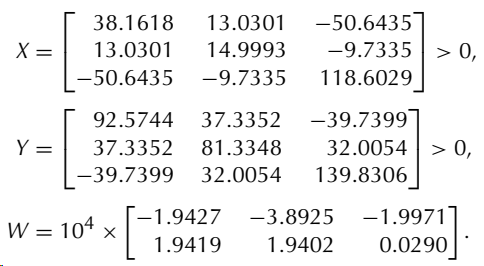
\includegraphics[width=0.7\linewidth]{Solution1/screenshot001}
		\caption[Exercise 1.2.5, Burden-Faires, 8ed.]{}
		\caption{}
		\label{fig:screenshot001}
	\end{figure}
\end{Solution}
 
   
\end{document}